\documentclass[12pt,a4paper]{article}
% The following LaTeX packages must be installed on your machine: amsmath, authblk, bm, booktabs, caption, dcolumn, fancyhdr, geometry, graphicx, hyperref, latexsym, natbib
\input{183.dat}
\usepackage{gensymb}
\usepackage{amsthm}
\usepackage{float}
\usepackage{siunitx}
\usepackage{amssymb}
\usepackage{float}
\usepackage{enumerate}
\usepackage{listings}
\usepackage{mathtools}
\PassOptionsToPackage{hyphens}{url}\usepackage{hyperref}
\usepackage[none]{hyphenat}
\usepackage{physics}
\newcommand\ddfrac[2]{\frac{\displaystyle #1}{\displaystyle #2}}
%\renewcommand{\familydefault}{\sfdefault}


\begin{document}

\setcounter{page}{1}

\section*{LE3 Problem 1}
\bigskip

Last 4 digits of phone number: 2256. $G(s)$ is

\begin{equation}
	G(s) = \frac{3}{2s^2 + 5s + 6} \label{eq:gs}
\end{equation}

Putting this into a unity-gain negative feedback gives

\begin{equation}
	H(s) = \frac{G(s)}{1 + G(s)} \label{eq:hs}
\end{equation}

Its response to a unit step function is shown in Fig. \ref{fig:hs-step}, with \%OS $= 10\%$ and $T_p = 1.83$ s. There is also a steady state error of $67\%$.

\begin{figure}[h!]
	\centering
	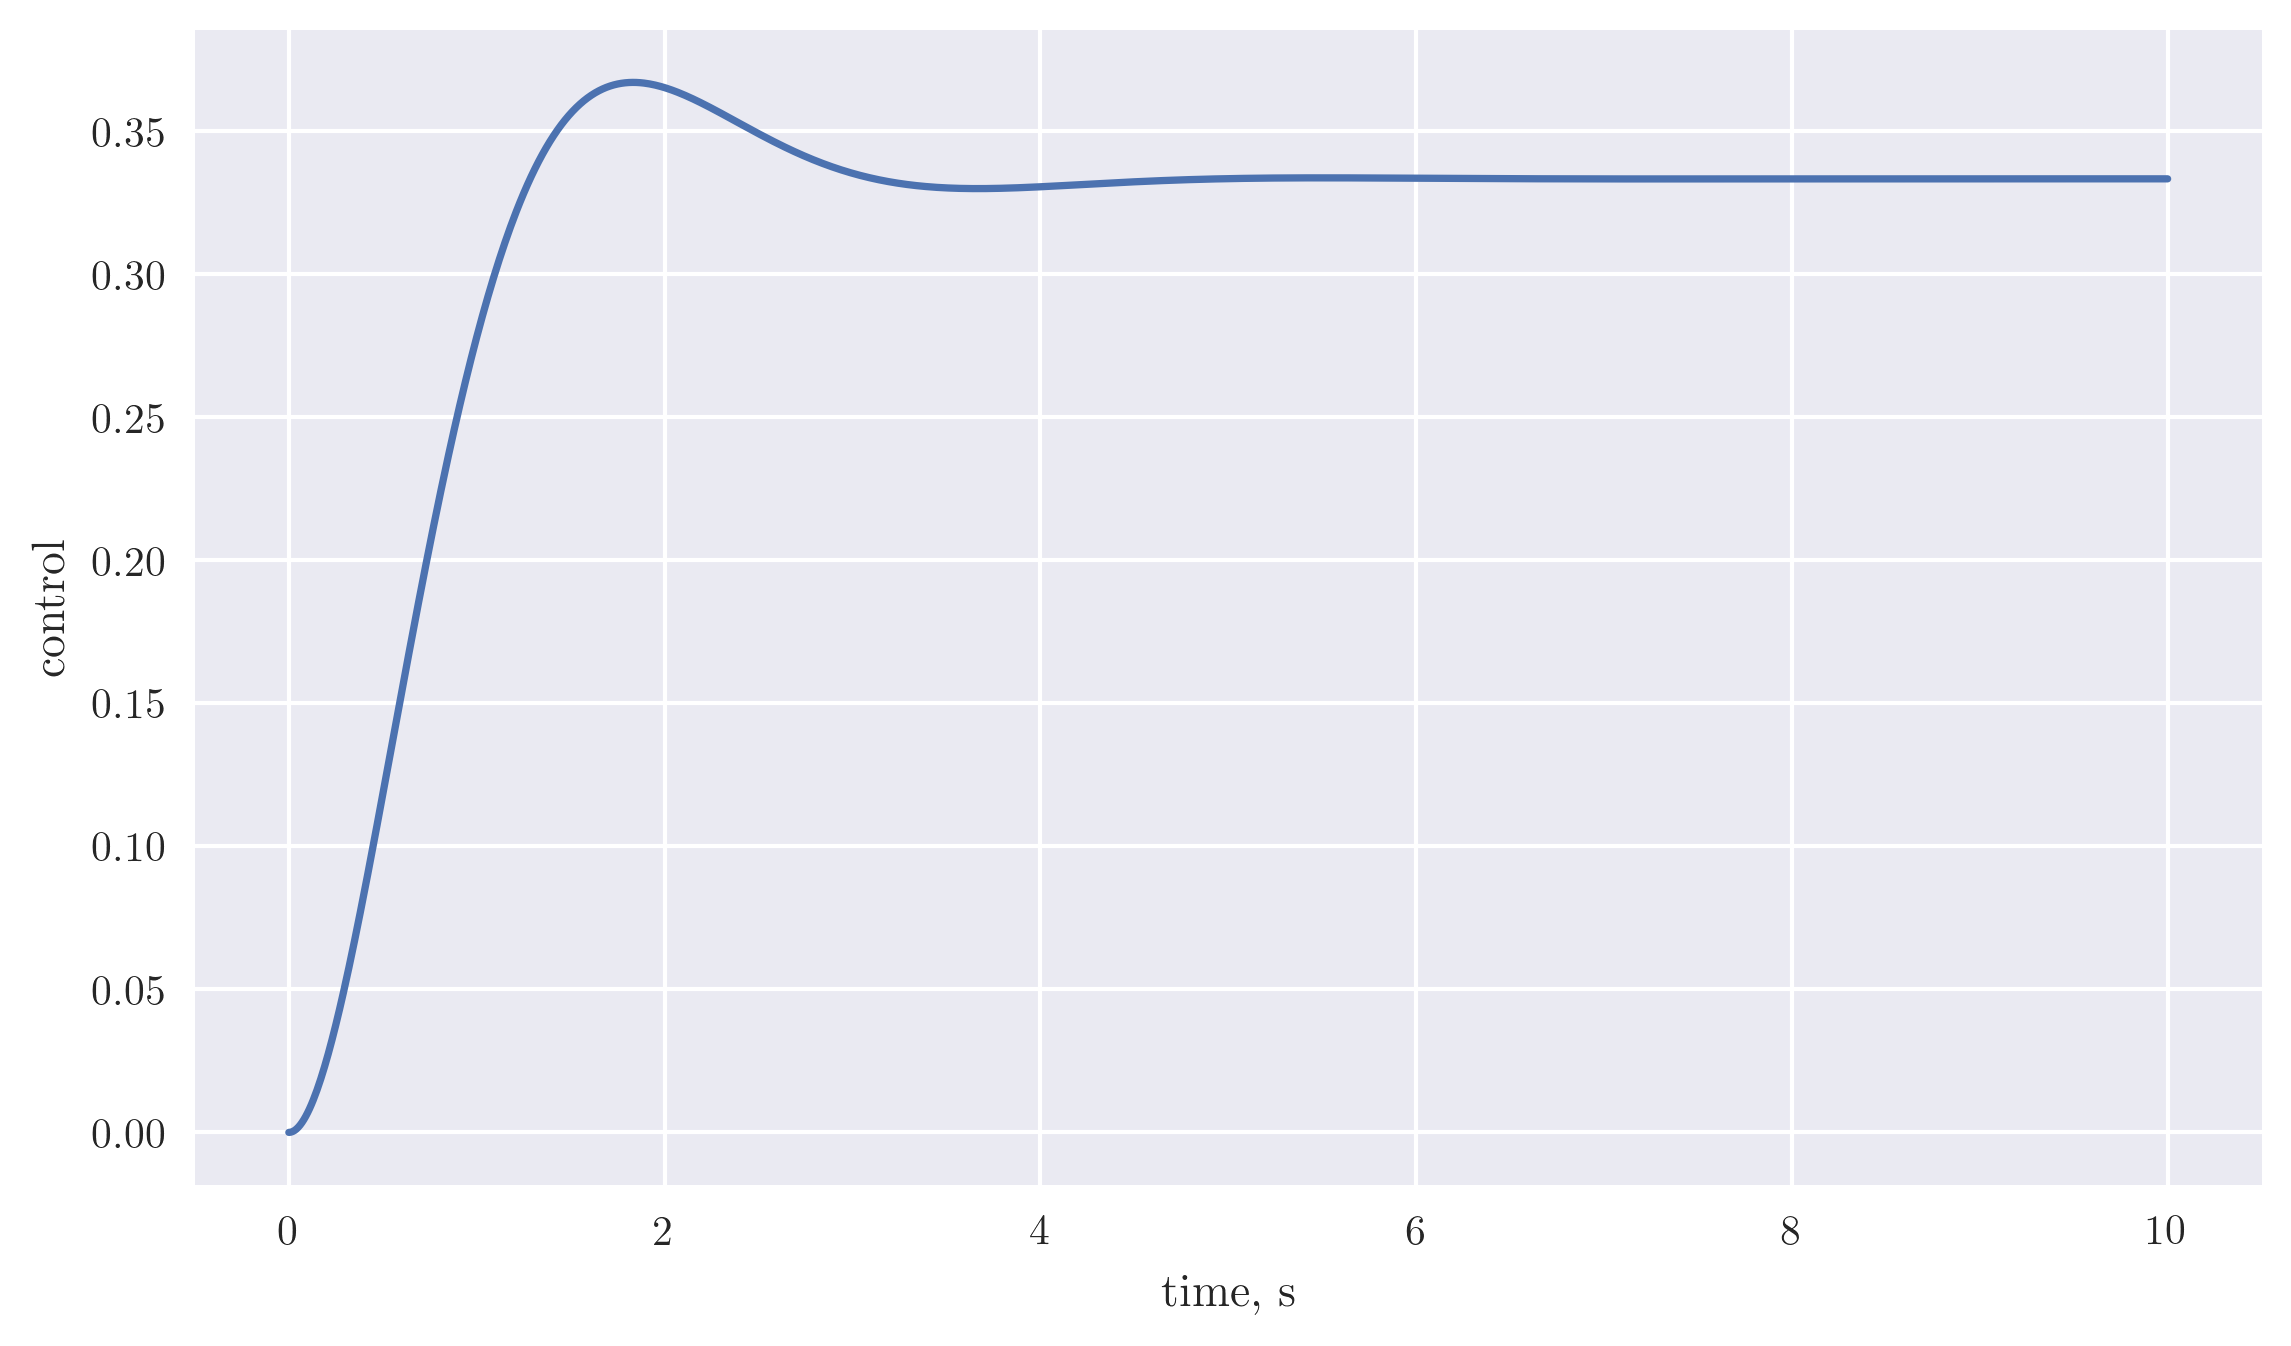
\includegraphics[width=0.75\linewidth]{LE3_gs_step.png}
	\caption{Response of $H(s)$ to a unit step function.}
	\label{fig:hs-step}
\end{figure}

We want a step response with a percent overshoot of at most 10\% and a peak time of 0.1 s.

\begin{enumerate}[a)]

\item \textbf{Desired pole location}

\begin{align}
	s_d &= -\sigma_d \pm j\omega_d \\
	&= \zeta\omega_n + j\omega_n\sqrt{1 - \zeta^2} \\
	\zeta &= \frac{-\ln(\%OS)}{\sqrt{\pi^2 + \ln^2(\%OS)}} \\
	&= \frac{-\ln(0.1)}{\sqrt{\pi^2 + \ln^2(0.1)}} \\
	&= 0.59 \label{eq:zeta}
\end{align}

\begin{align}
	\omega_n &= \frac{\pi}{T_p\sqrt{1 - \zeta^2}} \\
	&= \frac{\pi}{0.1\sqrt{1 - 0.59^2}} \\
	&= 38.95 \textrm{ rad/s} \label{eq:natural-frequency} \\
	s_d &= -(0.59)(38.95) + j(38.95)\sqrt{1 - (0.59)^2} \\
	\Aboxed{
		s_d &= -23.03 + 31.42j
	} \label{eq:sd}
\end{align}

\item \textbf{Angle deficiency}

\begin{align}
	G(s_d) &= \frac{3}{2s_d^2 + 5s_d + 6} \\
	&= -3.60\times 10^{-4} + 9.62\times 10^{-4} j \\
	\measuredangle G(s_d) &= \arctan(\frac{\Im[G]}{\Re[G]}) \\
	&= 1.92 \textrm{ rad} = 110.49^\circ \\
	\Phi_d &= \pi - \measuredangle G(s_d) \\
	\Aboxed{
		\Phi_d &= 1.21 \textrm{ rad}
	} \label{eq:angle-def}
\end{align}

\item \textbf{Compensator poles and zeros}

\begin{align}
	\alpha &= \arctan(\frac{1 - \zeta^2}{\zeta}) \\
	&= \arctan(\frac{1 - 0.59^2}{0.59}) \\
	&= 0.94 \\
	z_c &= -\omega_n \sqrt{1 - \zeta^2} \tan(\frac{\alpha - \Phi_d}{2}) - \zeta\omega_n \\
	&= -(38.95)\sqrt{1 - (0.59)^2} \tan(\frac{0.94 - 3.42}{2}) - (0.59)(38.95) \\
	\Aboxed{
		z_c &= -18.68
	} \label{eq:zc}
\end{align}

\begin{align}
	p_c &= -\omega_n \sqrt{1 - \zeta^2} \tan(\frac{\alpha + \Phi_d}{2}) - \zeta\omega_n \\
	&= -(38.95)\sqrt{1 - (0.59)^2} \tan(\frac{0.94 + 3.42}{2}) - (0.59)(38.95) \\
	\Aboxed{
		p_c &= -81.21
	} \label{eq:pc}
\end{align}

\item \textbf{Compensator gain}

\begin{align}
	K &= \ddfrac{1}{\abs{G(s_d)\frac{s_d + z_c}{s_d + p_c}}} \\
	&= \ddfrac{1}{\abs{(-3.60 \times 10^{-4} + 9.62 \times 10^{-4} j) \frac{-23.03 + 31.42j - 18.68}{-23.03 + 31.42j - 81.21}}} \\
	\Aboxed{
	K &= 2030.30
	} \label{eq:gain}
\end{align}

\item \textbf{Simulink implementation}

\begin{figure}[h!]
	\centering
	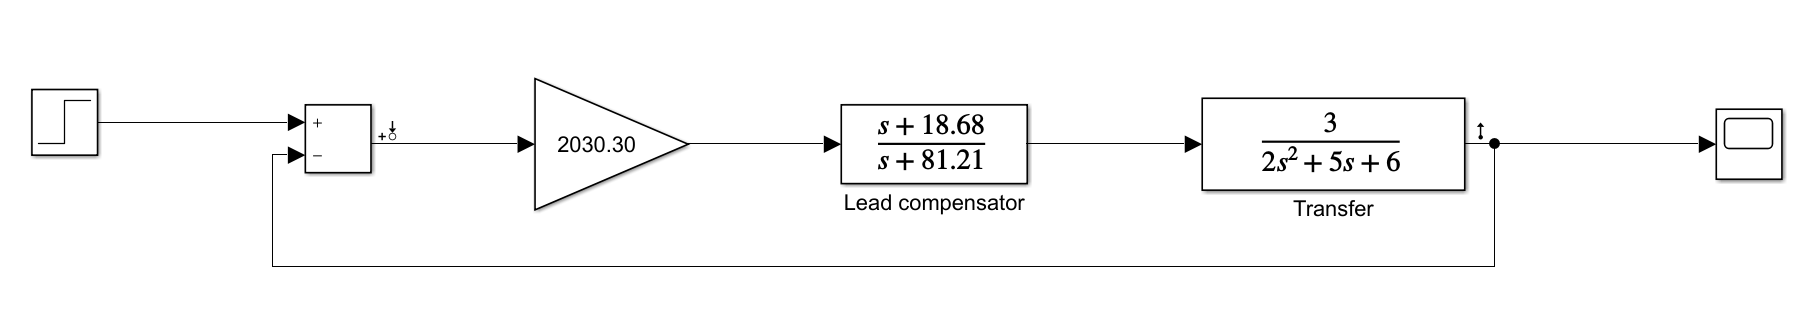
\includegraphics[width=\linewidth]{lc_simulink.png}
	\caption{Lead compensator implementation in MATLAB Simulink.}
	\label{fig:lc-simulink}
\end{figure}

\begin{figure}[h!]
	\centering
	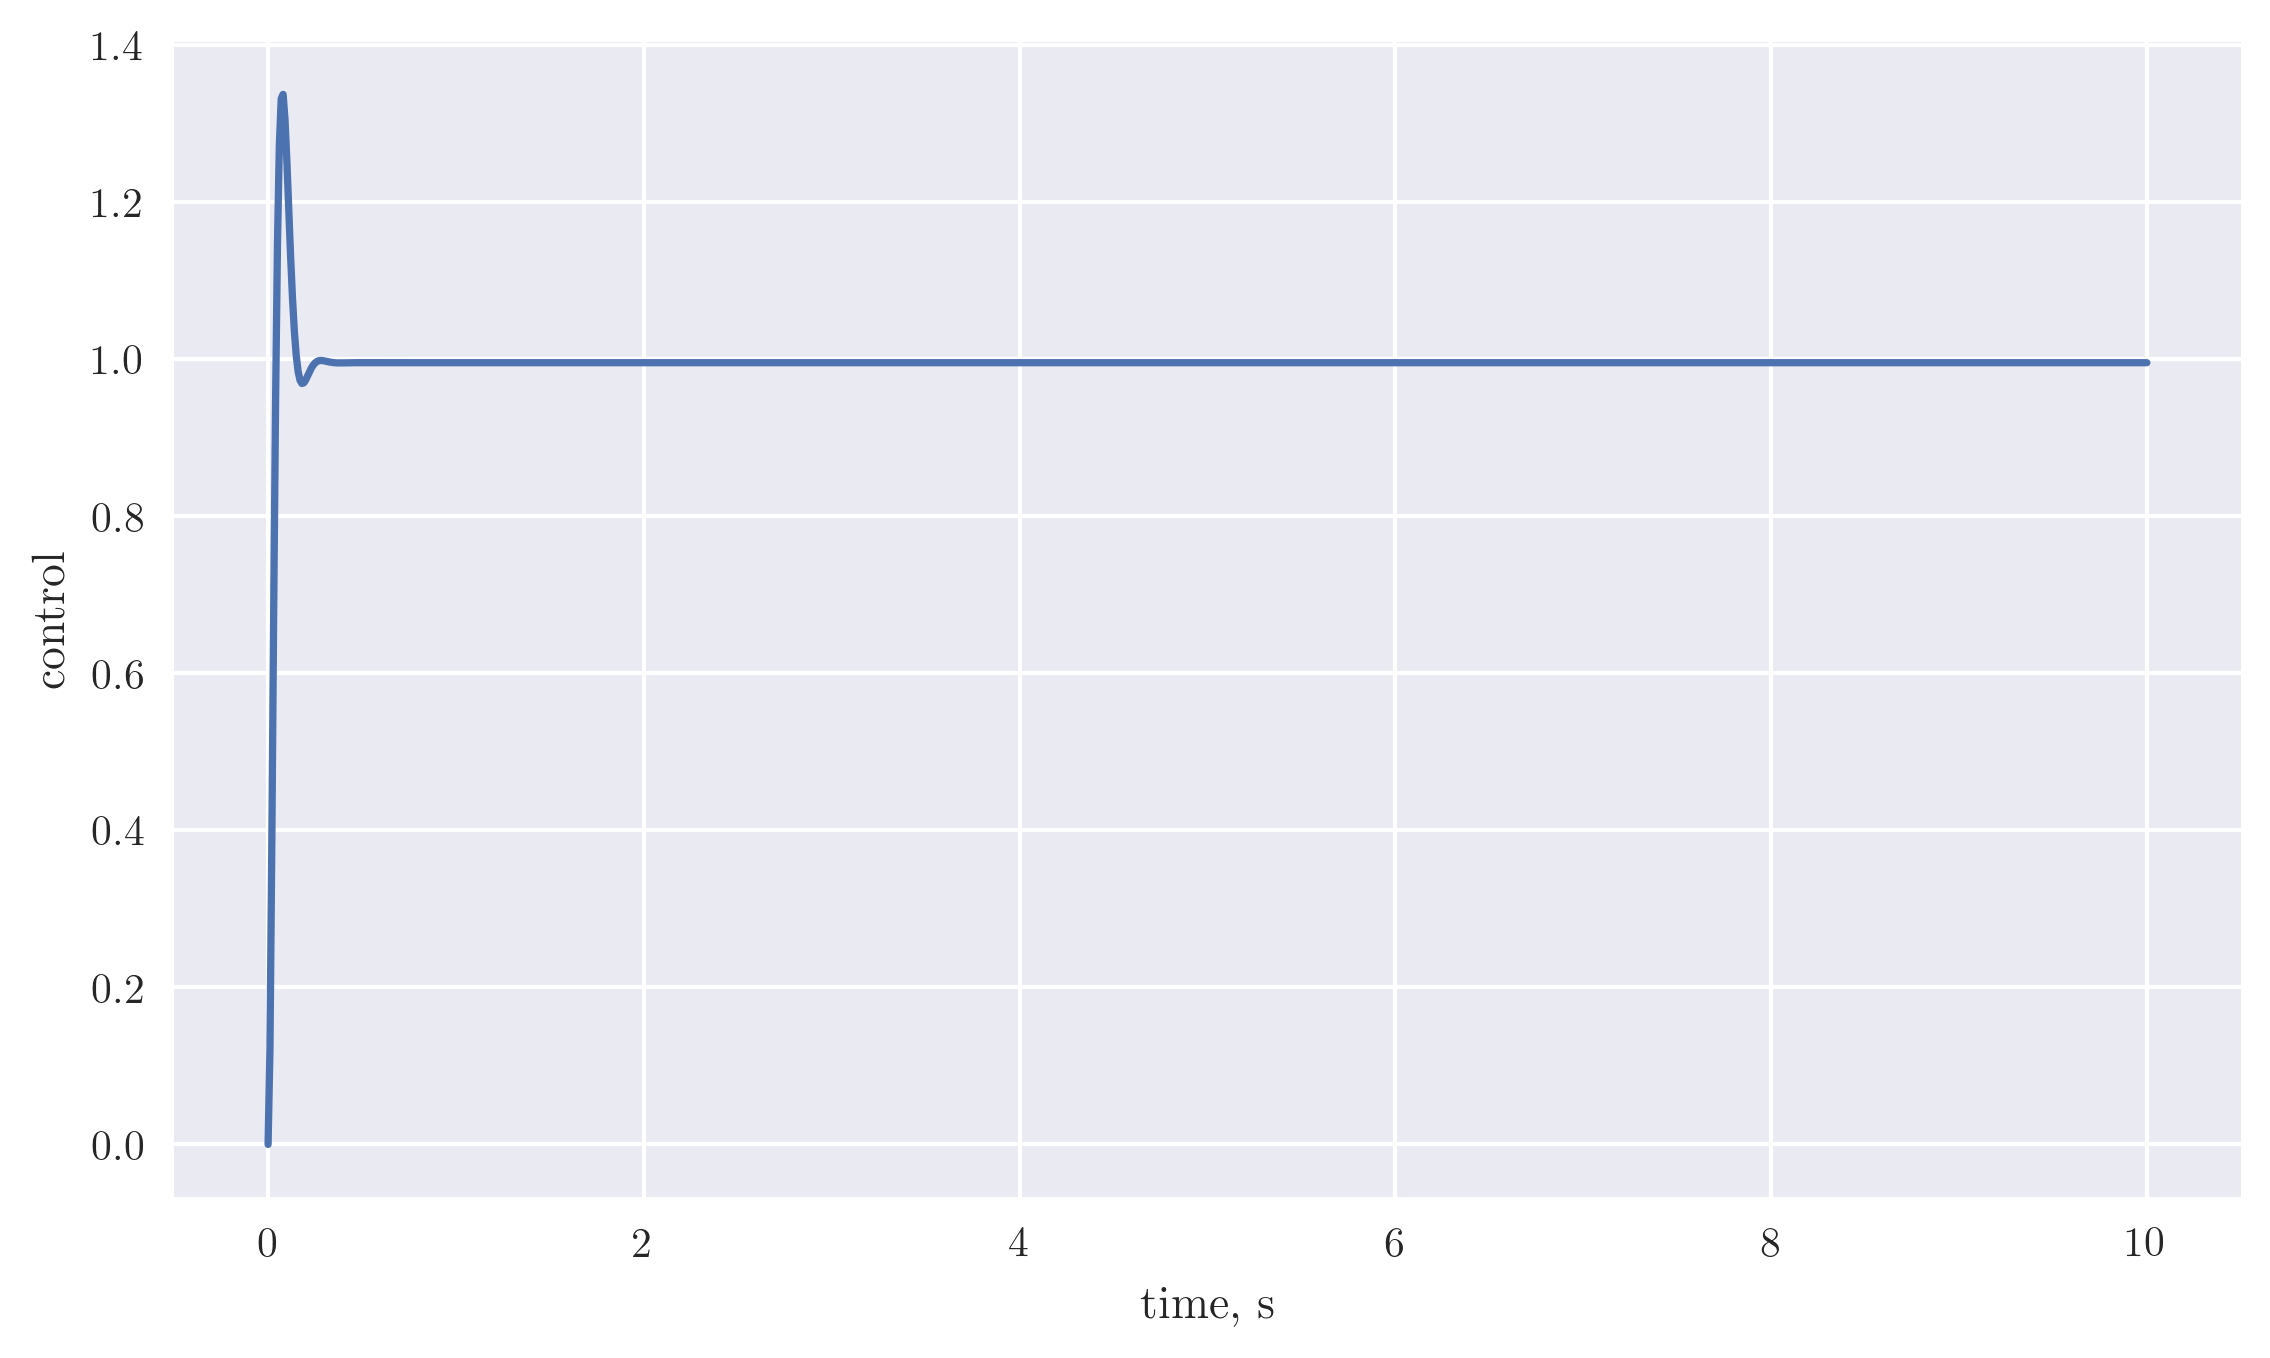
\includegraphics[width=0.9\linewidth]{LE3_lc_step.png}
	\caption{Unit step response of the system in Fig. \ref{fig:lc-simulink}.}
	\label{fig:lc-step}
\end{figure}

From Fig. \ref{fig:lc-step}, we have \%OS $= 34\%$ and $T_p = 0.08$ s. The lead compensator was able to bring the peak time slightly below 0.1 s, but actually increased the overshoot.

\end{enumerate}

\end{document}